\documentclass{article}[12pt]
\usepackage{graphicx}
\usepackage{float,times}
\usepackage{alltt}
\usepackage{moreverb}
\usepackage{url}
\usepackage{supertabular}

\floatstyle{ruled}
\newfloat{Code listing}{thp}{lop}[section]

%%%\renewcommand{\comment}[1]{}

\newcommand{\chebycoeff}{{\tt ChebyCoeff }}
\newcommand{\nsintegrator}{{\tt NSIntegrator }}
\newcommand{\flowfield}{{\tt FlowField }}
\newcommand{\dnsflags}{{\tt DNSFlags }}
\newcommand{\timestep}{{\tt TimeStep }}
\newcommand{\Vector}{{\tt Vector }}



\newcommand{\subsubsubsection}[1]{
\vspace{1mm}
\noindent
{\bf #1}
\vspace{1mm}
}
\newcommand{\Caption}[1]{\begin{singlespacing} \caption{#1} \end{singlespacing}}

\newcommand{\etal}{{\em et al.}}
\newcommand{\etalsp}{{\em et al.\ }}
\newcommand{\Rey}{\mbox{{\it Re}}}
\renewcommand{\Re}{\operatorname{Re}}
\renewcommand{\Im}{\operatorname{Im}}
\newcommand{\be}{{\bf e}}
\newcommand{\del}{\partial}
\newcommand{\tOmega}{\tilde{\Omega}}
\newcommand{\tpi}{\tilde{\pi}}
\newcommand{\cross}{\times}

\newcommand{\Nx}{{\tt Nx }}
\newcommand{\Ny}{{\tt Ny }}
\newcommand{\Nz}{{\tt Nz }}

\newcommand{\wtf}{\widetilde{f}}
\newcommand{\bu}{{\bf u}}
\newcommand{\bv}{{\bf v}}
\newcommand{\bff}{{\bf f}}
\newcommand{\bg}{{\bf g}}
\newcommand{\bB}{{\bf B}}
\newcommand{\ba}{{\bf a}}
\newcommand{\bA}{{\bf A}}
\newcommand{\bC}{{\bf C}}
\newcommand{\bc}{{\bf c}}
\newcommand{\bd}{{\bf d}}
\newcommand{\bQ}{{\bf Q}}
\newcommand{\bn}{{\bf n}}
\newcommand{\bx}{{\bf x}}
\newcommand{\bU}{{\bf U}}
\newcommand{\bR}{{\bf R}}
\newcommand{\bS}{{\bf S}}
\newcommand{\bH}{{\bf H}}
\newcommand{\bF}{{\bf F}}
\newcommand{\bL}{{\bf L}}
\newcommand{\bN}{{\bf N}}
\newcommand{\bomega}{{\boldsymbol \omega}}
\newcommand{\bPhi}{{\bf \Phi}}
\newcommand{\bPsi}{{\bf \Psi}}
\newcommand{\bphi}{{\boldsymbol \phi}}
\newcommand{\qqquad}{\qquad \quad}


\newcommand{\htbu}{\widehat{\widetilde{\bu}}}

\newcommand{\tU}{\tilde{U}}
\newcommand{\tV}{\tilde{V}}
\newcommand{\tW}{\tilde{W}}
\newcommand{\tP}{\tilde{P}}
\newcommand{\tu}{\tilde{u}}
\newcommand{\tv}{\tilde{v}}
\newcommand{\tw}{\tilde{w}}
\newcommand{\tx}{\tilde{x}}
\newcommand{\ty}{\tilde{y}}
\newcommand{\tz}{\tilde{z}}

\newcommand{\oU}{\overline{U}}
\newcommand{\what}[1]{\widehat{#1}}
%\renewcommand{\hat}[1]{\widehat{#1}}

\newcommand{\tot}[1]{#1_{\text{tot}}}
\newcommand{\butot}{\bu_{\text{tot}}}
\newcommand{\ptot}{p_{\text{tot}}}

%\newcommand{\tot}[1]{\underline{#1}}
%\newcommand{\butot}{\underline{\bu}}
%\newcommand{\ptot}{\underline{p}}

\newcommand{\hf}{\widehat{f}}
\newcommand{\hp}{\hat{p}}
\newcommand{\hq}{\hat{q}}
\newcommand{\hu}{\hat{u}}
\newcommand{\hv}{\hat{v}}
\newcommand{\hw}{\hat{w}}
\newcommand{\hN}{\hat{N}}
\newcommand{\hR}{\hat{R}}
\newcommand{\hbC}{\hat{\bC}}
\newcommand{\hbR}{\hat{\bR}}
\newcommand{\hbf}{\hat{\bff}}
\newcommand{\hbg}{\hat{\bg}}
\newcommand{\hPhi}{\hat{\Phi}}
\newcommand{\hbPhi}{\hat{\bPhi}}
\newcommand{\hPsi}{\hat{\Psi}}
\newcommand{\hbPsi}{\hat{\bPsi}}
\newcommand{\hbL}{\hat{\bL}}
\newcommand{\hbN}{\hat{\bN}}
\newcommand{\hbu}{\hat{\bu}}
\newcommand{\rN}{\bar{N}}
\newcommand{\nts}{\negthickspace}

\newcommand{\tp}{\tilde{p}}
\newcommand{\tq}{\tilde{q}}
\newcommand{\tN}{\tilde{N}}
\newcommand{\tR}{\tildehat{R}}
\newcommand{\tbC}{\tilde{\bC}}
\newcommand{\tbR}{\tilde{\bR}}
\newcommand{\tbf}{\tilde{\bff}}
\newcommand{\tPhi}{\tilde{\Phi}}
\newcommand{\tPsi}{\tilde{\Psi}}
\newcommand{\tbPsi}{\tilde{\bPsi}}
\newcommand{\tbL}{\tilde{\bL}}
\newcommand{\tbN}{\tilde{\bN}}
\newcommand{\tbu}{\tilde{\bu}}

\newcommand{\kron}{\delta}
\newcommand{\kxkz}{k_x,k_z}
\newcommand{\norm}[1]{\parallel #1 \parallel}
\newcommand{\bnabla}{{\bf \nabla}}
\newcommand{\grad}{{\bf \nabla}}
\newcommand{\tgrad}{\tilde{\bf \nabla}}
\newcommand{\tbnabla}{\tilde{\bf \nabla}}
\newcommand{\dvrg}{{\bf \nabla \cdot}}
\newcommand{\tdvrg}{\tilde{\bf \nabla} \cdot}
\newcommand{\lapl}{\nabla^2}
\newcommand{\tlapl}{\tilde{\nabla}^2}
\newcommand{\tavg}[1]{\langle #1 \rangle_t}
\newcommand{\mxzavg}[1]{\langle #1 \rangle_{mxz}}
\newcommand{\xzavg}[1]{\langle #1 \rangle_{xz}}
\newcommand{\tibu}{\tilde{\bu}}

\newcommand{\hgrad}{\what{\grad}}
\newcommand{\hlapl}{\what{\nabla}^2}

\newcommand{\eqn}[1]{eqn.\ \ref{#1}}
\newcommand{\eqns}[2]{eqns.\ \ref{#1} and \ref{#2}}
\newcommand{\Eqn}[1]{Eqn.\ \ref{#1}}
\newcommand{\Sec}[1]{Section \ref{#1}}
\newcommand{\sek}[1]{section \ref{#1}}
\newcommand{\fig}[1]{fig.\ \ref{#1}}
\newcommand{\Fig}[1]{Fig.\ \ref{#1}}

\newcommand{\F}[1]{\mathcal{F}_{#1}}
\newcommand{\Fk}{\mathcal{F}_{k_x k_z}}
\newcommand{\til}{\tilde{}}
\newcommand{\defn}{\triangleq}
\newcommand{\IP}[2]{\left(#1, #2\right)}
\newcommand{\IPO}[2]{\left(#1, #2\right)_{\Omega}}
\newcommand{\IPo}[2]{\left(#1, #2\right)_{\Omega'}}
\newcommand{\IPy}[2]{\left(#1, #2\right)_{L_y'}}
\newcommand{\IPY}[2]{\left(#1, #2\right)_{L_y}}
\newcommand{\VO}{V_{\Omega}}
\newcommand{\Vo}{V_{\Omega'}}

\newcommand{\dd}[1]{\frac{\partial}{\partial #1}}
\newcommand{\ddx}{\dd{x}}
\newcommand{\ddy}{\dd{y}}
\newcommand{\ddz}{\dd{z}}
\newcommand{\ddt}{\dd{t}}

\newcommand{\spann}{\operatorname{span}}
\newcommand{\cond}{\operatorname{cond}}
\newcommand{\rms}{\operatorname{RMS}}
\newcommand{\vol}{\operatorname{vol}}
%\newcommand{\exp}{\operatorname{exp}}
%\newcommand{\UAHLS}{U_{\text{A}}}
\newcommand{\UAHLS}{U_A}
%%% Local Variables: 
%%% mode: latex
%%% TeX-master: t
%%% End: 


\begin{document}

\renewcommand{\arraystretch}{1.5}

\title{Channelflow description}
\author{John F. Gibson\\jfg@member.fsf.org}
\maketitle

%\vspace{1in}
%\begin{centering}
%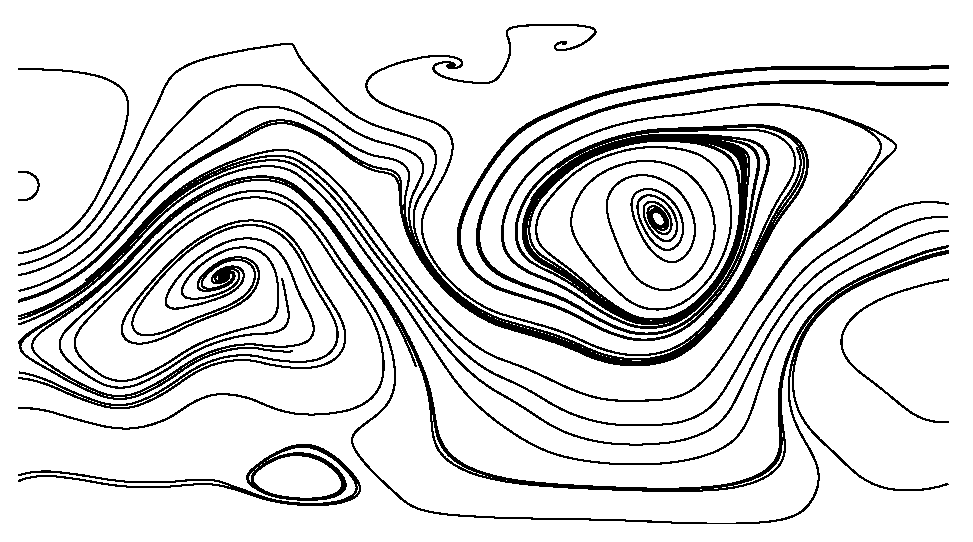
\includegraphics[height=3in]{streams.eps}
%\end{centering}
%\pagebreak
\thispagestyle{empty}
%\pagebreak
\indent

%\begin{abstract}
%\end{abstract}

Channelflow is a direct numerical simulator for incompressible fluid
flow on a periodic, rectangular, wall-bounded domain. Channelflow uses
spectral discretization in spatial directions (Fourier x Chebyshev x
Fourier), finite-differencing in time, and primitive variables (3d
velocity and pressure) to integrate the incompressible Navier-Stokes
equations. The mathematics are based on the spectral channel-flow
algorithm in Section 7.3 of {\em Spectral Methods in Fluid Dynamics}
by Canuto, Hussaini, Quarteroni, and Zang. Channelflow is written in
C++ and designed to be easy to use, easy to understand, modular,
extensible, and fast. Channelflow is documented, licensed under the
GNU GPL version 2, and available for download at

Channelflow is written as a set of C++ classes that represent the
major components of spectral channel-flow simulation. The channelflow
class library provides a high-level representation for expressing and
performing spectral channel-flow simulations. In channelflow's
high-level syntax, fluids simulation programs are short, readable, and
easily modifiable. Channelflow falls short of a providing a {\em
language} for spectral simulation, due to the scope of the problem
domain and to the difficulty of presenting a clean syntax through C++
class libraries. But channelflow should be good enough for a general 
use by fluids researchers who need a fast, simple, and extensible way 
to simulate channel flows.

Channelflow's classes are designed to be modular. Instances of classes
behave as independent objects with automatic memory management. 
Auxiliary fields and computations can be added to a program with a few
lines of code. In channelflow, even the DNS algorithm is an object. 
This greatly increases the flexibility of DNS computations. For
example, a DNS can be reparameterized and restarted multiple times
within a single program, multiple independent DNS computations can run
side-by-side within the same program, and DNS computations can run as
small components within a larger, more complex computations. As a
result, comparative calculations that formerly required coordination 
of several programs through shell scripts and saved data files can
be done within single channelflow program. In this way channelflow 
opens the way to a new class of computations that were not practically 
possible with previous codes.

Channelflow uses object-oriented programming and data abstraction to
maximize the organization and readability of its library code, as
well. Channelflow defines about a dozen C++ classes that act as
abstract data types for the major components of spectral channel-flow
simulation, as outlined by CHQZ. Each class forms a level of
abstraction in which a set of mathematical operations are performed in
terms of lower-level abstractions, from time-stepping equations at the
top to linear algebra at the bottom. The channelflow library code thus
naturally reflects mathematical algorithm, both in overall structure
and line-by-line. One can look at any part of the code and quickly 
understand what role it plays in the overall algorithm. One can learn 
the algorithm in stages, either top-down or bottom-up, by focusing 
on one level of abstraction at a time. 

Thus channelflow has three main benefits: 
\begin{itemize} 
\item {\bf Ease of use:} Channelflow's high-level syntax allows 
simple, rapid development of particular channel-flow simulations.
\item {\bf Modularity:} Its modularity allows a broader range of 
channel-flow computations.
\item {\bf Intelligibility:} Its library code is organized and 
documented in a way that makes learning the details easy.
\end{itemize}
Additional benefits are
\begin{itemize} 
\item {\bf Extensibility:} Channelflow is adaptable to new needs. For 
example, it should be easy to add a new time-stepping algorithm or 
method of calculating the nonlinear term. 
\item {\bf Speed:} Channelflow is as fast as comparable Fortran codes
\item {\bf Verifiability:} Channelflow contains a test suite 
that verifies the correct behavior of major classes.
\item {\bf Documentation:} The documentation describes how to use 
the software and precisely specifies the mathematics of the algorithm.
\item {\bf Support:} Channelflow has a support website 
with public CVS access, support-request and bug-tracking systems, etc.
(\url{http://savannah.nongnu.org/projects/channelflow}).
\end{itemize}


Channelflow is hosted at 
\begin{center}
\url{http://savannah.nongnu.org/projects/channelflow}
\end{center}

The latest source code and user's manual can be obtained at
\begin{center}
\url{http://savannah.nongnu.org/files/?group=channelflow}
\end{center}

\end{document}
